\documentclass{llncs}
% * <peter.christen@anu.edu.au> 2016-08-19T15:07:29.567Z:
%
% ^.
%\usepackage{llncsdoc}
\usepackage{epsfig}
\usepackage{graphicx}

%\usepackage{caption}
%\usepackage{subcaption}

\newtheorem{mydef}{Def.}
\newtheorem{myhyp}{Hypothesis}

\usepackage{url}
\usepackage{hyperref}

\pagestyle{empty}

% PAKDD 2017: maximum 12 pages
% Abstract max 200 words
% title, abstract: 1/2 page
% introduction: 1 1/2 page (2 pages so far)
% related work: 1 to 1 1/2 pages (3 pages so far)
% method: 4 pages (7 pages so far)
% experiments: 3 (10 pages so far)
% discussion /conclusion: 1 page
% citations 1

% ====================================================================

% Eamonn ICDM'10 tutorial slides
% - clear problem statement in abstract
% - To convince a reviewer, you must think like a reviewer

% Writing the paper:
% - Make a working title
% - Introduce the topic and define (informally at this stage)
%   terminology
% - Motivation: Emphasize why is the topic important
% - Relate to current knowledge: what’s been done
% - Indicate the gap: what need’s to be done?
% - Formally pose research questions
% - Explain any necessary background material.
% - Introduce formal definitions.
% - Introduce your novel algorithm/representation/data structure etc.
% - Describe experimental set-up, explain what the experiments will
%   show
% - Describe the datasets
% - Summarize results with figures/tables
% - Discuss results
% - Explain conflicting results, unexpected findings and discrepancies
%   with other research
% - State limitations of the study
% - State importance of findings
% - Announce directions for further research
% - Acknowledgements
% - References
%
% - Don’t make the reviewer of your paper think!
% - Reviewers make an initial impression on the first page and don’t
%   change 80% of the time
% - A good introduction with a good motivation is half your success
% - By the end of the introduction the reviewer mustknow.
%   - What is the problem?
%   - Why is it interesting and important?
%   - Why is it hard?why do naive approaches fail?
%   - Why hasn't it been solved before?(Or, what's wrong with previous
%     proposed solutions?)
%   - What are the key components of my approach and results?Also
%     include any specific limitations.
%   - A final paragraph or subsection: “Summary of Contributions”.
%     It should list the major contributions in bullet form,
%     mentioning in which sections they can be found. This material
%     doubles as an outline of the rest of the paper, saving space and
%     eliminating redundancy
% - Unjustified Choices (are bad)
% - Optimal: Does not mean `very good'
% - Proved: Does not mean `demonstrated'
% - Significant: There is a danger of confusing the informal statement
%   and the statistical claim
% - Use all the Space Available
% - Avoid Weak Language: aim, attempt, might, etc.
% - Use the Active Voice
% - ALWAYS put some variance estimate on performance measures (do
%   everything 10 times and give me the variance of whatever you are
%   reporting)

% Figures:
% - Don't cover the data with the labels!
% - Color helps -Direct labeling helps -Meaningful captions help
%
% Common problem with figures:
% 1.Too many patterns on bars
% 2.Use of both different symbols and different lines
% 3.Too many shades of gray on bars
% 4.Lines too thin (or thick)
% 5.Use of three-dimensional bars for only two variables
% 6.Lettering too small and font difficult to read
% 7.Symbols too small or difficult to distinguish
% 8.Redundant title printed on graph
% 9.Use of gray symbols or lines
% 10.Key outside the graph
% 11.Unnecessary numbers in the axis
% 12.Multiple colors map to the same shade of gray
% 13.Unnecessary shading in background
% 14.Using bitmap graphics (instead of vector graphics)
% 15.General carelessness

% ====================================================================

% TODO:
% - clearly point out novelty of this work
% - contribution compared to earlier work

\begin{document}

% ideas for a better shorter title?
\title{Efficient Cryptanalysis of Bloom Filters for
       Privacy-Preserving Record Linkage
  \thanks{The authors would like to thank the Isaac Newton Institute
  for Mathematical Sciences, Cambridge, for support and hospitality
  during the programme \emph{Data Linkage and Anonymisation} where
  this work was conducted (EPSRC grant EP/K032208/1). Peter Christen
  was also supported by a grant from the Simons Foundation. The work
  was also partially funded by the Australian Research Council
  (DP130101801).}}

\author{Peter Christen\inst{1} \and Rainer Schnell\inst{2}
        \and Dinusha Vatsalan\inst{1} \and Thilina
        Ranbaduge\inst{1}}
\institute{Research School of Computer Science,
           The Australian National University, \\
           Canberra, Australia.~
           Contact: \email{peter.christen@anu.edu.au}
           \and
           Methodology Research Group, %Institute for Sociology,
           University Duisburg-Essen, Duisburg, Germany.} %~
%           \email{rainer.schnell@uni-due.de}}

\maketitle

\begin{abstract}
Privacy-preserving record linkage (PPRL) is the process of identifying
records that represent the same entity across databases held by
different organizations without revealing any sensitive information
about these entities. A popular technique used in PPRL is Bloom
filter encoding, which has shown to be an efficient and effective way
to encode sensitive information into bit vectors while still enabling
approximate matching of attribute values. However, the encoded values
in Bloom filters are vulnerable to cryptanalysis attacks. Under
specific conditions, these attacks are successful in that some
frequent sensitive attribute values can be re-identified.
%
%While previous attacks have high computational requirements
In this paper we propose and evaluate on real databases a novel
efficient attack on Bloom filters. Our approach is based on the
construction principle of Bloom filters of hashing elements of sets
into bit positions. The attack is independent of the encoding
function and its parameters used, it can correctly re-identify
sensitive attribute values even when various recently proposed
hardening techniques have been applied, and it runs in a few seconds
instead of hours.
\end{abstract}

\keywords Privacy; re-identification; frequency analysis; data
          linkage.

% ====================================================================

\section{Introduction}
\label{sec-intro}

Integrating data from different sources with the aim to remove
duplicates, enrich data, and correct errors and inconsistencies is a
crucial data pre-processing task for many data mining and analytics
applications~\cite{Chr12}. Example applications include healthcare,
business analytics, national censuses, population informatics, fraud
detection, government services, and national security.

However, growing concerns about privacy and confidentiality
increasingly preclude the exchange or sharing of personal identifying
attributes, such as names, dates of birth, and addresses, which are
generally required for linking databases due to the non-existence of
common unique entity identifiers~\cite{Chr12,Vat13}. Work in
privacy-preserving record linkage (PPRL) aims to develop techniques
for identifying records that correspond to the same entity across
several databases while not compromising the privacy and
confidentiality of the entities~\cite{Vat13}.

PPRL is achieved by conducting linkage on the encoded (masked) values
of the identifying attributes of records across two or more databases.
%~\cite{Fie05}.
%
Several data encoding techniques for PPRL have been developed. These
can be categorized into cryptographic secure multi-party computation
(SMC) and perturbation-based techniques~\cite{Vat13}. The former are
accurate and provably secure, but they incur expensive computation
and communication costs.
%The latter category includes more efficient techniques which often
%provide a trade-off between accuracy and privacy.
%Since existing cryptographic-based techniques are not scalable for
%real applications,
Most PPRL techniques are therefore based on perturbation-based
techniques that provide adequate privacy protection while achieving
acceptable linkage quality~\cite{Ran16,Vat13}.

Bloom filter (BF) encoding is one such perturbation-based technique
that has successfully been used in several recent practical PPRL
applications~\cite{Boy15,Ran14}. A BF is a binary vector with bits
initially set to $0$. 
%with bits set to $0$ or $1$. As we describe in detail in
%Sect.~\ref{sec-overview},
A value can be encoded into a BF using a set of hash functions by
setting corresponding bits to $1$~\cite{Sch09}, and the approximate
similarity between two BFs can be calculated by counting the number
of positions where both BFs have $1$-bits in common.

% Peter: I don't think this next paragraph is needed for this paper
% as it is not needed to understand the paper
%The similarity (or distance) between a pair of values is preserved in
%the BF space such that the similarity calculated using their BF
%encodings is greater than or equal to the similarity calculated using
%their unencoded values. BF-based similarity calculation allows false
%positives due to collision of bits (where different values are
%hash-mapped into the same bit) which improves the privacy aspect
%while compromising accuracy (depending on the false positive rate).
%Therefore, it is crucial to set the BF related parameters ($k$, $l$,
%and number of elements to be hash-mapped into a BF) appropriately to
%balance the accuracy and privacy aspects of
%linkage~\cite{Sch09,Vat16}.

As we discuss in detail in the next section, BFs can be susceptible
to cryptanalysis attacks that aim to re-identify the encoded
sensitive attribute values~\cite{Kro15,Kuz11,Kuz13,Nie14}. Using 
frequency counts and patterns in a set of BFs, these attacks
iteratively map bit patterns to known attribute values. These existing
attacks are however not practical as they require knowledge of certain
parameters used during the BF encoding phase, and they have high
computational costs.

Our contribution in this paper is an efficient frequency-based
approach for attacking BFs that exploits the fundamental property of
how the elements of sets are hashed into BFs, as we describe in
Sect.~\ref{sec-overview}. In contrast to existing attack methods, our
novel approach does not require any assumption on the BF parameters
used when sensitive attribute values were encoded. It is also
significantly faster, making it a viable attack on large sets of
BFs to evaluate whether they provide adequate privacy protection. We
experimentally evaluate our attack method on two real-world data
sets, showing its efficiency and effectiveness.

Given BF encoding is now being employed in real-world PPRL
applications~\cite{Boy15,Ran14}, it is crucial to study possible
attacks on BFs to ensure their security and to make users of such
systems aware of the weaknesses of BF encoding. Our novel attack
method allows data custodians to identify such weaknesses of BF
encoding that otherwise could be exploited by an attacker.
%if appropriate BF encodings and parameters are not employed.

%Maybe add: Contributions:
%We propose a novel and efficient BF attack method and analyze its
%complexity

% PC 17/01/2107 until here **************************

% --------------------------------------------------------------------

\section{Prior Attacks on Bloom Filter based PPRL}
\label{sec-related}

%Bloom filters (BFs)~\cite{Blo70} are commonly used for the encoding of
%records in PPRL due to their capability of computing
%similarities~\cite{Dur14,Ran16,Sch09,Vat13}.
Schnell et al.~\cite{Sch09} were the first to introduce an
approximate matching approach for PPRL using Bloom filters (BFs), as
we describe in detail in Sect.~\ref{sec-overview}. A recent study by
Randall et al.~\cite{Ran14} has shown that PPRL based on BF encoding
can achieve similar linkage quality as can be achieved with
traditional linkage methods on the unencoded attribute values. As a
result, BF encoding has been the PPRL technique of choice in several
recent practical PPRL applications~\cite{Boy15,Ran14}.
%
%However, BFs are prone to different
%attacks~\cite{Kro15,Kuz11,Kuz13,Nie14} which will be described %shortly.
%
However, BFs are prone to different
attacks~\cite{Kro15,Kuz11,Kuz13,Nie14}. Therefore, a comprehensive
analysis of the weaknesses of BFs in the PPRL context is required. We
now describe the few studies that have been conducted on attacks on
BFs.

% From Dinusha's introduction:
%An attack using a constraint satisfaction solver was studied by
%Kuzu et al.~\cite{Kuz11,Kuz13}, where values are mapped to bit
%patterns that meet constraints such as frequency alignments. A
%successful attack on BFs using filtering and statistical analysis
%techniques was recently investigated by Niedermeyer et
%al.~\cite{Nie14}. Based on the linear combination of the values used
%to generate hash functions, this attack first generates a set of
%possible bit patterns (so called \emph{atoms}) that are then aligned
%according to their frequencies with known attribute
%values~\cite{Nie14}. 

Kuzu et al.~\cite{Kuz11} formulated a cryptanalysis attack on BFs
as a constraint satisfaction problem (CSP). CSP is characterized by
a set of variables and a set of constraints on these variables. The
aim of this attack is to identify a set of values from a given domain
that can be assigned to each variable such that the constraints are
satisfied. This is achieved by a frequency analysis of the sensitive
attribute values and the BF encodings of the records in a database.
However, this attack requires that the attacker has access to a
global database where the encoded records are drawn from. This
is unlikely in practical applications.

In 2013, Kuzu et al.~\cite{Kuz13} investigated the accuracy of their
CSP attack with two real-world databases. The authors tried to
re-identify the personal details of patients in an encoded medical
database by using a frequency analysis of BF encodings of a public
voter registration database that has a different frequency
distribution to the medical database. Their results indicated that
although the CSP attack might be feasible in such situations, it is
less likely to be accurate in identifying original attribute
values and it requires more computational resources. The attack
re-identified four out of 20 frequent names correctly.

% Peter: results below are different to Table 1? *******************

Niedermeyer et al.~\cite{Nie14} more recently proposed an attack on
BFs built from German surnames. The attack was based on the
frequencies of sub-strings of length 2 extracted from frequent
surnames. Of $7,580$ surnames, the authors re-identified the $934$
most frequent ones (about $12\%$) before stopping the attack. In
contrast to the approach in~\cite{Kuz13}, this attack only 
%is not based on the assumption that the attacker has
%access to a population data set from which the surnames are drawn.
%However, the feasibility of this approach 
depends on the availability of a list of the most common surnames.
This work was extended by Kroll and Steinmetzer~\cite{Kro15} into a
cryptanalysis on BF encodings of several attributes, which was able
to re-identify $44\%$ of all attribute values correctly. However, both
attacks are based on the specific double hashing scheme used by
Schnell at al.~\cite{Sch09}.

Existing cryptanalysis attacks are feasible only for certain
settings and assumptions used in the BF encoding phase. They also
require excessive computational resources making them not practical
in real settings. Our novel attack method, described next, improves
on both these drawbacks of existing methods.

% --------------------------------------------------------------------

\begin{figure}[t]
  \centering
  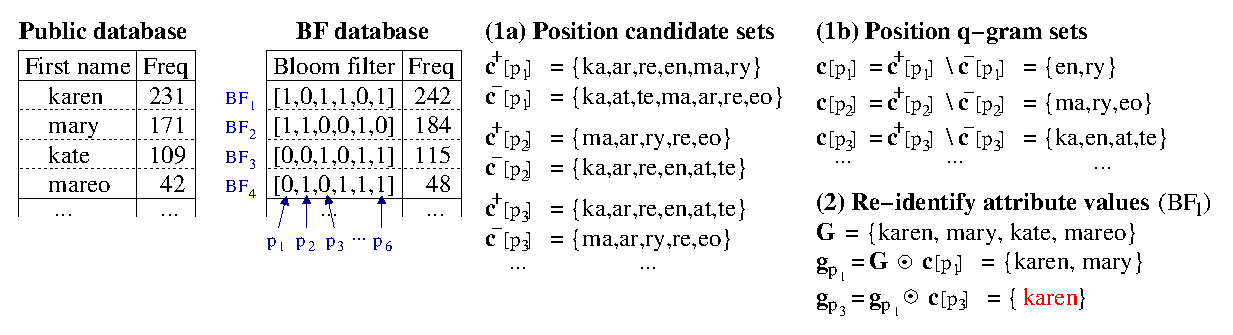
\includegraphics[width=1.0\textwidth]{bf-attack-outline}
  \caption{Outline of the proposed cryptanalysis attack, which is
           based on a set of BFs and a set attribute values, both
           sorted according to their frequencies. In steps (1a) and
           (1b), the attack exploits the bit patterns in BFs to
           identify the sets of q-grams that are possible,
           $\mathbf{c}^+[p]$, and \emph{not} possible,
           $\mathbf{c}^-[p]$, respectively, for each bit position
           $p$. In step (2), the re-identification of a set of
           (sensitive) attribute values, $\mathbf{G}$, is conducted
           by intersecting the q-gram sets of values in $\mathbf{G}$
           with the sets $\mathbf{c}$ (illustrated using $\odot$).
           %as outlined in Sect.~\ref{sec-overview} and detailed in
           %Sect.~\ref{sec-bf-attack}.
           \label{fig:outline}}
\end{figure}

\section{Overview and Preliminaries}
\label{sec-overview}

We now provide an overview of our attack on BFs, as illustrated in
Fig.~\ref{fig:outline}. As with other attacks on
BFs~\cite{Kro15,Kuz11,Kuz13,Nie14}, our approach exploits the
frequency distribution of a set of BFs that were generated from a
large database. As for notation, we use bold letters for sets
(with upper-case bold letters for lists or sets of sets) and normal
type letters for integer or string values. We denote sets with curly
and lists with square brackets, where lists have an order while sets
do not.

We assume the attacker has access to a set of encoded BFs,
$\mathbf{B}$, and their frequencies, but he does not know anything
about the parameters used in the encoding process (such as the number
of hash functions used, or the actual hashing mechanism). We assume
these BFs represent a set of records that encode sensitive values
from one or a few attributes. Based on the frequency distribution of
the Hamming weights (number of $1$-bits) in $\mathbf{B}$, the attacker
can guess which attribute(s) have been encoded, because different
attributes (such as first name, surname, city name, or postcode) have
distinctive distributions of Hamming weights~\cite{Sch16}. The
distribution of Hamming weights is independent of the (unknown)
secret key. Therefore, an attacker can sample attribute values from
a publicly available population database (such as a telephone
directory) and select a set of frequent values, $\mathbf{V}$, from
an attribute that has a frequency distribution that is similar to
the distribution of the set to be attacked.
%matches with the distribution
%of the set of BFs $\mathbf{B}$ to be attacked.

In step (1), we first align BFs and attribute values according to
their frequencies, and consider the set of most frequent values in 
both. For each bit position $p$ in the BFs,
%of length $l$ (with $1 \le p \le l$),
for all corresponding attribute values that have this bit set to $1$
we add their q-grams (sub-strings of length $q$ generated from
attribute values) to the set $\mathbf{c}^+[p]$ of possible
q-grams for that position. The reasoning is that a $1$-bit means at
least one q-gram of an attribute value was hashed to this position.
For all attribute values with a value of $0$ at bit
position $p$ we add their q-grams to the set $\mathbf{c}^-[p]$ of
\emph{not} possible q-grams for that position, because a $0$-bit
means no q-gram of an attribute value could have been mapped to this
position.

At the end of step (1), for each position $p$ we obtain the set
$\mathbf{c}[p] = \mathbf{c}^+[p] \setminus \mathbf{c}^-[p]$ of
q-grams that potentially could have been hashed to position $p$.
Based on the list $\mathbf{C} = [\mathbf{c}[1], \ldots,
\mathbf{c}[l]]$, where $l$ is the length of the BFs, and a set
$\mathbf{G}$ of attribute values we aim to re-identify (i.e.\ learn
which BF possibly encodes which value in $\mathbf{G}$), in step (2)
we analyze each BF in $\mathbf{B}$ and remove those attribute values
from $\mathbf{G}$ that are not possible matches according to
$\mathbf{C}$ because they do not contain any q-grams that would have
been hashed to a certain $1$-bit.

For example, in Fig.~\ref{fig:outline}, for the most frequent BF$_1$,
`kate' is not a possible value because in order to obtain a $1$-bit
in position $p_1$, it would have to contain either the q-gram `en'
or `ry'; while `mary' is also not possible because it would need to
contain one of the q-grams `ka', `en', `at', or `te' in position
$p_3$.

Before we formalize and present our approach in detail in
Sect.~\ref{sec-bf-attack}, we first describe BF encoding, as well as
some recent approaches to harden them.

% - - - - - - - - - - - - - - - - - - - - - - - - - - - - - - - - - -

\smallskip

%\subsection{Bloom Filter Encoding}
%\label{sec-bf-encoding}

\begin{figure}[!t]
  \centering
  %\scalebox{1.0}[1.0]
  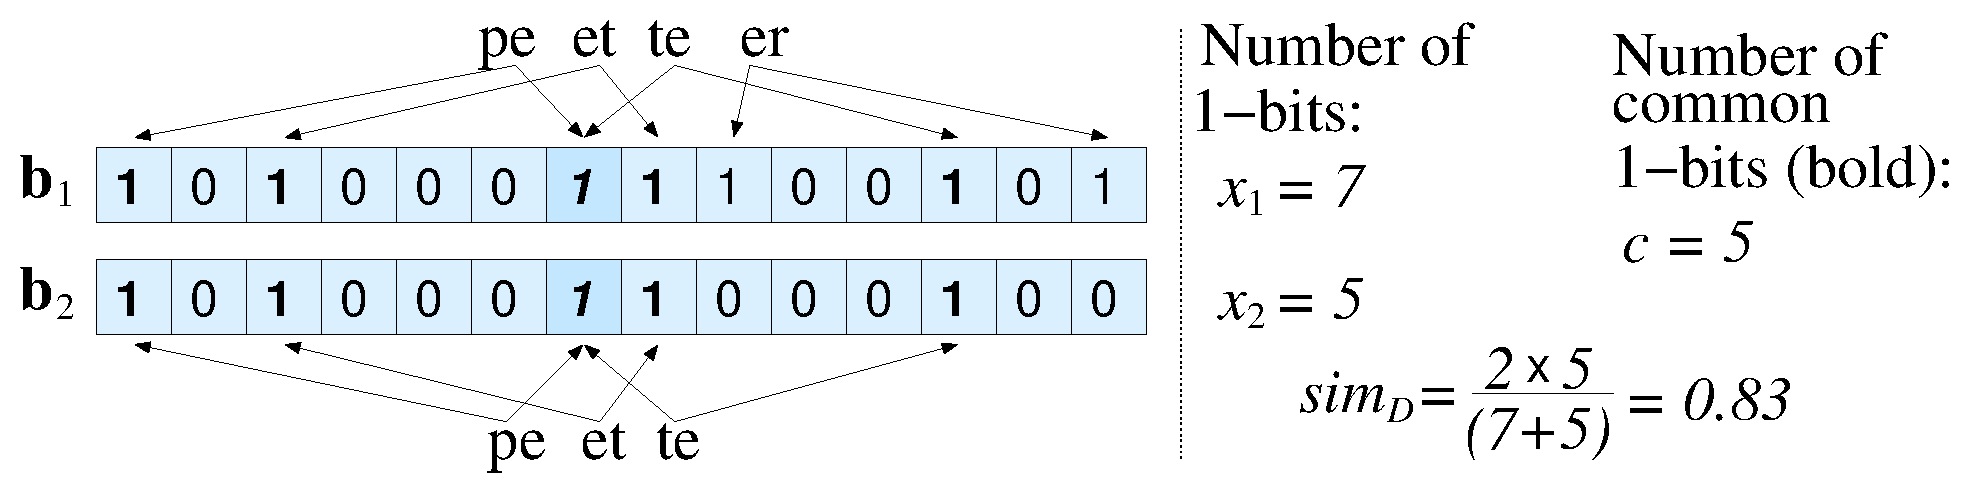
\includegraphics[width=0.65\textwidth]{bloomfilter}
  \caption{An example Dice coefficient similarity calculation of the
           two first names `peter' and `pete'  encoded in BFs, as
           described in Sect.~\ref{sec-overview}. The dark bit shows
           a hash collision.}
           \label{fig:bloomfilter}
\end{figure}

\textbf{Bloom Filter Encoding:}~
Proposed by Bloom~\cite{Blo70} in 1970 for the space and time
efficient representation of sets, a BF $\mathbf{b}$ is a bit vector
of length $l$ where all bits are initially set to $0$. $k$
independent hash functions, $h_1, \ldots, h_k$, each with range
$1, \ldots, l$, are used to map the elements $s$ in a set
$\mathbf{s}$ into the BF by setting the bit positions
$\mathbf{b}[h_j(s)]=1$, with $1 \le j \le k$.

For PPRL, the set $\mathbf{s}$ of q-grams generated from string
values~\cite{Sch09}, or neighboring values for numerical
values~\cite{Vat16}, can be hash-mapped into a BF. These BFs are then
either sent to a linkage unit (LU, an external party that conducts
the linkage) to calculate the similarity between BFs in order to
classify them as matches or non-matches~\cite{Sch09}, or they are
partially exchanged among the database owners to distributively
calculate the similarities between BFs~\cite{Vat14c}.

%Any set-based similarity function (such as Overlap, Jaccard, and Dice
%coefficient~\cite{Chr12}) can be used to calculate the similarity of
%pairs or sets of (multiple) BFs.

The Dice coefficient has been used for comparing BFs since it is
insensitive to many matching zeros
%(bit positions to which no elements are hash-mapped)
in long BFs~\cite{Sch09}. 
%
For two BFs, $\mathbf{b}_1$ and $\mathbf{b}_2$, the Dice coefficient
similarity is: $sim_D(\mathbf{b}_1, \mathbf{b}_2) = 2  c / (x_1 +
x_2)$,
%\begin{eqnarray}
%\label{eq:Dice_coefficient}
%sim_D(\mathbf{b}_1, \mathbf{b}_2) &=& \frac{2 \times c}{x_1 + x_2},
%\end{eqnarray}
where $c$ is the number of bit positions that are set to $1$ in both
BFs (common $1$-bits), and $x_1$ and $x_2$ are the number of bit
positions set to $1$ in $\mathbf{b}_1$ and $\mathbf{b}_2$,
respectively.
%
Figure~\ref{fig:bloomfilter} shows the encoding of bigrams ($q=2$)
of two string values into $l=14$ bits long BFs using $k=2$ hash
functions, and their Dice coefficient similarity calculation.

Different encoding methods have been proposed for BFs. Hashing
several attributes of a record into one BF is a method known as
cryptographic long term key (CLK). It is used to improve
privacy~\cite{Sch11}. Another record-level BF encoding (RBF) was
proposed to improve linkage quality~\cite{Dur14}. In RBF,
attribute values are first hashed into different BFs and then bits
are selected from each attribute-level BF into a RBF according to
attribute weights.

The initial proposal of BFs for PPRL used a double hashing
scheme~\cite{Sch09}, where the $k$ individual bit positions for an
element $s$ to be hashed are determined by the sum of the integer
representation of two independent hash functions that are mapped into
the range $1-l$. Random hashing has recently been proposed as an
improvement over double hashing to prevent against cryptanalysis
attacks, where $k$ random numbers are drawn for every element $s$ to
be hashed~\cite{Nie14,Sch16}.

%  - - - - - - - - - - - - - - - - - - - - - - - - - - - - - - - - - -

\smallskip

%\subsection{Bloom Filter Hardening}
%\label{sec-bf-harden}

\textbf{Bloom Filter Hardening:}~
Several BF hardening methods have been studied in recent times to
reduce the vulnerability of BFs against cryptanalysis
attacks~\cite{Sch16}. Compared to attribute-level BFs, record-level
BF encodings such as CLK and RBF reduce the risk of re-identification
by such attacks~\cite{Kuz11,Nie14}.

Exploiting the fact that data sets with (near) uniform Hamming
weight distribution of BFs are more difficult to attack (with
existing attack methods) than data sets with non-uniform
distributions, balancing BFs with constant Hamming weight has been
proposed~\cite{Sch16}. Balanced BFs can be constructed by
concatenating a BF of length $l$ with its negated copy (all bits
flipped) and then permuting the $2l$ bits. Another proposed approach
to harden BFs is XOR-folding, where a BF of length $l$ is split into
two halves of length $l/2$ each, and then bit-wise exclusive OR is
applied to combine the two shorter BFs~\cite{Sch16}.

While balancing and XOR-folding are easy and data independent
hardening techniques, salting with record-specific values has been
suggested as an alternative hardening method where an additional
(record-specific) value is concatenated with attribute values
before being hashed into the BF~\cite{Nie14}. A cryptanalysis attack
is unlikely to be successful without knowing the salting key, however
attributes suitable for salting might not be available in a database.
Other, more experimental hardening techniques, include random bits
and fake record injection~\cite{Dur14,Vat13}, as well as BLIP
(BLoom-and-flIP) which flips bits (noise addition) in a BF according 
to a differential privacy model~\cite{Sch16}. Many of these
hardening techniques improve security against attacks at the cost
of a reduction in linkage quality~\cite{Sch16}. In the experiments
in Sect.~\ref{sec-data} we will investigate if balancing and
XOR-folding make BFs more resistant to our proposed attack.

% --------------------------------------------------------------------

\section{Frequency-based Bloom Filter Cryptanalysis}
\label{sec-bf-attack}

% define problem? or define problem in sect 3?

% below explain what we aim to achieve

% I think we need to explain that our attack does better than simply
% sorting attribute values and BF by frequencies and aligning
% them! we do find which q-grams are at which position

We now describe our frequency-based attack on BFs in detail. As shown
in Fig.~\ref{fig:outline}, the attack consists of two main steps.
First, for each BF position we find its set of possible and
\emph{not} possible q-grams
%$p$, $1 \le p \le l$, we find its set of possible q-grams,
%$\mathbf{c}[p]$
(steps (1a) and (1b) in Fig.~\ref{fig:outline}).
%
Next, 
%using the list $\mathbf{C} = [\mathbf{c}[1], \ldots, \mathbf{c}
%[l]]$,
we re-identify for each BF  
%in $\mathbf{B}$
the set of attribute values
% $g_i$ from a set of values $\mathbf{G}$
that possibly were hashed into this BF (step (2) in
Fig.~\ref{fig:outline}).
%
Algorithms~1 and~2 show the details of steps (1a) and (1b), and (2),
respectively, which we describe in the next two sub-sections. We then
provide an analysis of our attack and discuss its limitations.

%  - - - - - - - - - - - - - - - - - - - - - - - - - - - - - - - - - -

\subsection{Candidate Q-gram Set Generation}
\label{sec-cand-q-gram}

For our attack we require as input a set of BFs, $\mathbf{B}$, that
we assume to come from a sensitive database (the one from which we
aim to re-identify its sensitive values), and a set of attribute
values, $\mathbf{V}$, assumed to come from a public database. Each BF
$\mathbf{b}_i \in \mathbf{B}$ and each attribute value $v_i \in
\mathbf{V}$ has a frequency attached to it, denoted with
$\mathbf{b}_i.f$ and $v_i.f$, respectively. Unlike previous attacks on
BFs~\cite{Kuz11,Kuz13,Nie14}, we do not require any other information
about how the BFs were encoded.

\begin{figure}[t]
  \begin{center}
  \begin{scriptsize}
%    \begin{footnotesize}
  \begin{tabular}{ll} \hline
\multicolumn{2}{l}{\textbf{Algorithm 1: \emph{Candidate q-gram set
  generation}} -- Steps (1a) and (1b) } \\ \hline
\multicolumn{2}{l}{Input:} \\
\multicolumn{2}{l}{- $\mathbf{V}$: Set of attribute values and their
  frequencies from a public database} \\
\multicolumn{2}{l}{- $\mathbf{B}$: Set of BFs and their
  frequencies from the sensitive database} \\
\multicolumn{2}{l}{- $l$:~\, Length of Bloom filters} \\
\multicolumn{2}{l}{- $q$:~ Length of sub-strings to extract from
  attribute values} \\  
\multicolumn{2}{l}{- $m$: Minimum frequency for BFs and attribute
  values} \\
\noalign{\smallskip}
\multicolumn{2}{l}{Output:} \\
\multicolumn{2}{l}{- $\mathbf{C}$: List of possible q-grams for each
  BF position} \\
\noalign{\smallskip}
  1:  & $\mathbf{c}^+[p] = \{\}$, $\mathbf{c}^-[p] = \{\}$,
        $1 \le p \le l$ ~~~ // Initialize list of candidate q-gram
        sets \\
  2:  & $\mathbf{V}_F = \{v \in \mathbf{V}: v.f \ge m \}$
        ~~~~~~~~~~~~~~ // Attribute values with frequency of at
        least $m$ \\
  3:  & $\mathbf{B}_F = \{\mathbf{b} \in \mathbf{B}:
        \mathbf{b}.f \ge m \}$
        ~~~~~~~~~~~~~~\,// BFs with frequency of at least $m$ \\
  4:  & $revSort(\mathbf{B}_F)$, $revSort(\mathbf{V}_F)$ ~~~~~~~~~~ 
        // Sort according to frequencies, highest first \\
  5:  & $\mathbf{A} = [(\mathbf{b}_i, v_i) : 
        \mathbf{b}_i \in \mathbf{B}_F, v_i \in \mathbf{V}_F:
        \mathbf{b}_i.f > \mathbf{b}_j.f \land v_i.f > v_j.f:
        1 \le i < j \le min(|\mathbf{V}_F |, |\mathbf{B}_F|)]$ \\
  ~  &   ~~~~~~~~~~~~~~~~~~~~~~~~~~~~~~ // Align $\mathbf{V}_F$
        and $\mathbf{B}_F$ as long as their frequencies are
        unique \\  
  6:  & \textbf{for} $(\mathbf{b}_i, v_i) \in \mathbf{A}$
        \textbf{do}: ~~~~~~~~~~~~~~~~~~~~ //  Step (1a): Get
        candidate sets of q-grams \\
  7:  & ~~~ $\mathbf{q}_i = genQGramSet(v_i, q)$ ~~~~~~~~\,//
        Convert attribute value into its q-gram set \\
  8:  & ~~~  \textbf{for} $1 \le p \le l$ \textbf{do}: 
        ~~~~~~~~~~~~~~~~~~~\, // Loop over all BF positions \\
  9:  & ~~~ ~~~ \textbf{if} $\mathbf{b}_i[p] == 1$ \textbf{then}:
        ~~~~~~~~~~~~\, // Bit at position p is 1 \\
  10: & ~~~ ~~~ ~~~ $\mathbf{c}^+[p] = \mathbf{c}^+[p] \cup
        \mathbf{q}_i$ ~~~~~~~~~~~\,// Add to set of possible
        q-grams \\
  11: & ~~~ ~~~ \textbf{else}: ~~~~~~~~~~~~~~~~~~~~~~~~~~~~~~~~ //
        Bit at position $p$ is $0$ \\
  12: & ~~~ ~~~ ~~~ $\mathbf{c}^-[p] = \mathbf{c}^-[p] \cup
        \mathbf{q}_i$  ~~~~~~~~~~~// Add to set of \emph{not}
        possible q-grams \\
  13: & $\mathbf{C} = [\,]$ ~~~~~~~~~~~~~~~~~~~~~~~~~~~~~~~~~~~~~\,
        // Step (1b): Initialize empty list of q-gram sets \\
  14: & \textbf{for} $1 \le p \le l$ \textbf{do}: 
        ~~~~~~~~~~~~~~~~~~~~~~~~\,// Loop over all BF positions to
        combine q-gram sets \\
  15: & ~~~ $\mathbf{C}.append(\mathbf{c}^+[p] \setminus
        \mathbf{c}^-[p])$ ~~~~~~~~~~~\,// Remove not possible from
        possible q-grams \\
%  15: & ~~~ $\mathbf{c}[p] = \mathbf{c}^+[p] \setminus
%        \mathbf{c}^-[p]$ ~~~~~~~~~~~~~~~~~ // Remove not possible
%        from possible q-grams \\
%  16: & ~~~ $\mathbf{C}.append(\mathbf{c}[p])$
%        ~~~~~~~~~~~~~~~~~~~~~~ // Add to list of candidates for all
%        BF positions\\
16: & \textbf{return} $\mathbf{C}$ \\
  \hline
  \end{tabular}
%  \end{footnotesize}
 \end{scriptsize}
  \end{center}
  \label{algo:step1}
\end{figure}

Algorithm~1 starts by initializing two empty sets for each BF
position $p$: $\mathbf{c}^+[p]$ of possible q-grams at that
position, and $\mathbf{c}^-[p]$ of \emph{not} possible q-grams at
that position. Next, in lines 2 and 3, we find all BFs and attribute
values that occur at least $m$ times. In line 4 we sort both the BFs
and attribute values according to their frequencies in reverse order
(most frequent first), and then we align a BF $\mathbf{b}_i$ and an
attribute value $v_i$ into the sorted list $\mathbf{A}$ of pairs
$(\mathbf{b}_i, v_i)$. We do this as long as both the $i$th BF
$\mathbf{b}_i$ and $i$th attribute value $v_i$ have a unique
frequency compared to the next, less frequent, BF or attribute
value, respectively. This stopping criterion ensures that we do not
have a BF that could correspond to two or more attribute values,
and vice versa, as this would lead to more uncertainty in the
mapping of q-grams into BF positions.

Step (1a) of our approach starts in line 6 and loops over pairs of
aligned BFs and attribute values, $(\mathbf{b}_i, v_i) \in
\mathbf{A}$. First, we convert $v_i$ into its set of q-grams,
$\mathbf{q}_i$, in line 7. Then we loop over all BF positions,
$1 \le p \le l$, in line 8, and if the bit at position $p$ in BF is
$1$  (i.e., $\mathbf{b}_i[p] = 1$), we add the q-gram set
$\mathbf{q}_i$ to the set $\mathbf{c}^+[p]$ of possible q-grams at
that position (line 10) because a $1$-bit means any q-gram from
$\mathbf{q}_i$ could have been hashed to that position. Conversely,
if the BF bit at position $p$ is $0$, then no q-gram from
$\mathbf{q}_i$ could have been hashed to that position and so we add
the q-grams in $\mathbf{q}_i$ to $\mathbf{c}^-[p]$ (line 12).

In step (1b), line 13 onwards in Algo.~1, we get the final set of
q-grams for each BF position $p$ as the set of possible q-grams
($\mathbf{c}^+[p]$) minus the set of not possible q-grams
($\mathbf{c}^-[p]$), and add these sets to the list %of q-gram sets
$\mathbf{C}$ in line 15.

%  - - - - - - - - - - - - - - - - - - - - - - - - - - - - - - - - - -

\subsection{Attribute Value Re-identification}
\label{sec-reidentify}

\begin{figure}[t]
  \begin{center}
  \begin{scriptsize}
%    \begin{footnotesize}
  \begin{tabular}{ll} \hline
\multicolumn{2}{l}{\textbf{Algorithm 2: \emph{Attribute value
  re-identification}} -- Step (2) } \\ \hline
\multicolumn{2}{l}{Input:} \\
\multicolumn{2}{l}{- $\mathbf{B}$: Set of BFs from the sensitive
  database (same as in Algo.~1)} \\
\multicolumn{2}{l}{- $\mathbf{C}$: List of possible q-grams for
  each BF position (from Algo.~1)} \\
  \multicolumn{2}{l}{- $\mathbf{G}$: Set of attribute values we aim
  to re-identify in the set of BFs $\mathbf{B}$} \\
\noalign{\smallskip}
\multicolumn{2}{l}{Output:} \\
\multicolumn{2}{l}{- $\mathbf{R}$: List of possible attribute values
  re-identified for each BF in $\mathbf{B}$} \\
\noalign{\smallskip}
  1:  & $\mathbf{R} = [\,]$ ~~~~~~~~~~~~~~~~~~~~ // Initialize empty
        list of re-identified attribute values \\
%  1:  & $\mathbf{Q} = [\,]$ ~~~~ // Initialize empty list of q-gram
%        sets and attribute values \\
%  2:  & \textbf{for} $v_i \in \mathbf{G}$ \textbf{do}: ~~~~~~
%      // Loop
%      over all attribute values \\
%  3:  & ~~~ $\mathbf{q}_i = genQGramSet(v_i, q))$ ~ // Convert
%        attribute value into its q-gram set \\
%  4:  & ~~~ $\mathbf{Q}.append((\mathbf{q}_i, v_i))$ \\
  2:  & \textbf{for} $\mathbf{b}_i \in \mathbf{B}$
        \textbf{do}: ~~~~~~~~~ // Loop over all BFs \\
  3:  & ~~~ $\mathbf{g}_i = \mathbf{G}$ ~~~~~~~~~~~~~~~ //
        Initialize set of candidate attribute values as all
        possible values \\        
  4:  & ~~~  \textbf{for} $1 \le p \le l$ \textbf{do}: 
        ~~~~~~~~~~~~~~~~~~~~~~~\, // Loop over all BF positions \\
  5:  & ~~~ ~~~ \textbf{if} $\mathbf{b}_i[p] == 1$ \textbf{then}:
        ~~~~~~~~~~~~~~~~ // Bit at position $p$ is 1 \\
  6:  & ~~~ ~~~ ~~~ $\mathbf{c} = \mathbf{C}[p]$  ~~~~~~~~~~~~~~~~
        ~~~~~~~~~\, // Set of possible q-grams at this bit position
        \\
  7:  & ~~~ ~~~ ~~~ \textbf{for} $v_j \in \mathbf{g}_i$ \textbf{do}: 
        ~~~~~~~~~~~~~~~~~~~// Check all candidate attribute
        values \\
  8:  & ~~~ ~~~ ~~~ ~~~ \textbf{if} $(\forall q \in \textbf{c}:
        q \notin v_j)$ \textbf{then}: ~ // Check if no q-gram from
        $\mathbf{c}$ in attribute value \\
  9:  & ~~~ ~~~ ~~~ ~~~ ~~~ $\mathbf{g}_i = \mathbf{g}_i \setminus
        v_j$ ~~~~~~~~~~~~~~~\,// Value could not have been hashed
        into this BF \\ 
  10: & ~~~ $\mathbf{R}.append(\mathbf{g}_i)$ ~~~~~~~~~~~~~~~~~~~~~
        ~~~~~~ // Append possible attribute values for this BF \\
  11: & \textbf{return} $\mathbf{R}$ \\
  \hline
  \end{tabular}
%    \end{footnotesize}
  \end{scriptsize}
  \end{center}
  \label{algo:step2}
\end{figure}

The re-identification step, shown in Algo.~2, has as input the same
set of BFs, $\mathbf{B}$, as used in the first step, as well as the
list of candidate q-grams sets, $\mathbf{C}$, generated in Algo.~1.
A set of frequent attribute values, $\mathbf{G}$, also needs to be
provided. These are the values we aim to re-identify (guess) in
$\mathbf{B}$ using $\mathbf{C}$ (as shown in
Fig.~\ref{fig:outline}). The output of the algorithm is a set
of one or more re-identified attribute value(s), $\mathbf{g}_i
\subset \mathbf{G}$, for each BF $\mathbf{b}_i \in \mathbf{B}$,
collected in the result list $\mathbf{R}$.

The algorithm loops over all BFs $\mathbf{b}_i$ in $\mathbf{B}$ (line
2 onwards), and for each $\mathbf{b}_i$ it initializes the set of
possible candidate attribute values $\mathbf{g}_i$ (that potentially
have been hashed into this BF) as all values in $\mathbf{G}$ (line 3).
Next we loop over all BF positions $p$ (line  4), and for any position
that has a $1$-bit ($\mathbf{b}_i[p] = 1$) we retrieve the set of
possible q-grams $\mathbf{c} = \mathbf{C}[p]$ at that position
(line 6).

Using $\mathbf{c}$, we now check for each attribute value $v_j$ in
$\mathbf{g}_i$ if \emph{at least one of the q-grams} in $\mathbf{c}$
occurs in that value (lines 7 and 8). If $v_j$ does not contain at
least one q-gram from $\mathbf{c}$, it could not have generated the
$1$-bit at position $p$. If this is the case, in line 9 we remove
$v_j$ from the set of candidates $\mathbf{g}_i$. At the end of this
loop (line 10), the set $\mathbf{g}_i$ will contain all attribute
values from $\mathbf{G}$ that possibly have generated the BF
$\mathbf{b}_i$, and we append this set to the results list
$\mathbf{R}$. Note that positions with $0$-bits do not help us to
remove values $v_j \in \mathbf{g}_i$ because any q-gram in a value
$v_j$ is potentially hashed into other positions.
% Peter: not sure if this makes sense, we need to think further

%\textbf{\emph{In Algo.~2, we do not consider in a bit position $p$
%is $0$ (i.e. no else for the if in line 5). Are we missing something
%here? Would $0$-bits allow us to do more filtering? Can you please
%all have a think and let me know.. if there is nothing we can do with
%$0$-bits we should add a sentence why we cannot use them in the
%description of Algo.~2 below.}}

%% old below, PC 19/10 *****************************************

% Peter: Old and notes below,  maybe we can use somewhere:

%As with earlier attacks on BF-based PPRL approaches~\cite{...}, we
%assume that BFs are generated attribute-wise rather than record-wise,
%allowing us to analyze the frequency distribution of BFs as correlated
%with the frequency distribution of attribute values.

%Many attribute types commonly used in record linkage, such as first
%and last name, town or city names, postcodes or zipcodes, exhibit
%highly skewed frequency distributions of their values~\cite{?}. Often
%these distributions follow a Zipf-like distribution~\cite{}, where a
%few values occur very frequently (like surname `Smith' and `Miller' in
%English speaking countries), while the majority of values occur only
%rarely or once.

%As described in details below, we align the most frequent BFs from a
%set of BFs with the most frequent attribute values. We assume that
%an initial analysis of BF frequencies and attribute value frequencies
%(as shown in Fig.~\ref{xx}) has allowed us to identify which set of
%BFs corresponds to which attribute.

%Unlike other attack methods (which assume an attack knows certain
%parameters of the encoding approach used to generate the BFs~\cite{}),
%our attack does not require any such knowledge, making the attack more
%applicable and successful in situations where an attack only gains
%access to a set of BFs.

%Our attack exploits the fundamental properties of BFs: if a certain
%bit in a BF is not set to 1, then a corresponding element (q-gram in
%our case) of the set used to generate the BF cannot be in the %corresponding record.
%
%Using the alignment of frequent BFs and frequent attribute values,
%for each bit position of the BF we generate two sets: (1) the set of
%potential q-grams that \emph{cannot} be mapped to this position based
%on the q-grams in the frequent attribute values, and (2) the set of
%potential q-grams that \emph{can} be mapped to this position based on
%the q-grams in the frequent attribute values.

%- should we include how we find which BF correspond to which 
%  attributes? \\
% or is this an assumption? In section experiments we can show
% frequency plots of attributes and corresponding BF to show this
% step is easy
%
%- should we include the estimation of the number of hash functions k?
%  it is not too accurate at the moment, and somewhat independent of
%  our approach.

%  - - - - - - - - - - - - - - - - - - - - - - - - - - - - - - - - - -

\subsection{Analysis and Limitations}

\label{sec-analysis}
We now discuss the complexity and limitations of our cryptanalysis
attack.
\smallskip

\textbf{Complexity:}
We assume $N = |\mathbf{B}|$ is the number of BFs coming from the
sensitive database, $Q$ is the average number of q-grams per value
in the set of attribute values $\textbf{V}$ from the public
database, $k$ is the number of hash functions used to hash q-grams
into BFs, and $l$ is the length of a BF.

In step (1) of our attack, we first find all frequent BFs and
attribute values that occur at least $m$ times. This requires a
linear scan through $\mathbf{B}$ and $\textbf{V}$, respectively,
which has a complexity of $O(N)$ and $O(|\textbf{V}|)$. In line 4 of
Algo.~1, the sorting function used on values in $\textbf{B}_F$ and
$\textbf{V}_F$ has a complexity of $O(M \cdot log\,M)$, where $M =
min(|\textbf{B}_F|, |\textbf{V}_F|)$.
%
In step (1a), each attribute value in $\textbf{A}$ is converted into
its set of q-grams which are then added to the sets $\mathbf{c}^+[p]$
and $\mathbf{c}^-[p]$ for all BF bit positions $1 \le b \le l$. This
step has a computational complexity of $O(M \cdot Q \cdot l)$. In
step (1b), the sets of possible q-grams are added to list
$\mathbf{C}$ by performing a set difference operation between
$\mathbf{c}^+[p]$ and $\mathbf{c}^-[p]$. Assuming $\mathbf{Q}$ is
the set of all unique q-grams generated from all values $v_i \in
\mathbf{V}$, then on average $t=|\mathbf{Q}|*k/l$ q-grams are hashed
into each bit position. Therefore each set difference is of $O(t)$,
and so step (1b) has an overall complexity of $O(t \cdot l)$ for $l$
bit positions.
%The memory requirements of our algorithm is of $O(\mathbf{C})$ at
%the end of step 1.

In step (2) of our attack, Algo.~2 iterates through each BF
$\mathbf{b}_i \in \mathbf{B}$ to re-identify the possible attribute
values $\mathbf{g}_i \in \mathbf{G}$ that map to $\mathbf{b}_i$. For
each bit position $p$ that is set to $1$, we check if any q-gram in
$\mathbf{C}[p]$ occurs in a value $v_j \in \mathbf{g}_i$. This leads
to a total complexity of $O(N \cdot |\mathbf{G}| \cdot l \cdot t)$,
assuming the average size of a $\mathbf{C}[p]$ is $t$. Finally, the
worst case space complexity of the list $\mathbf{R}$ returned by
Algo.~2 is $O(N \cdot |\mathbf{G}|)$ if every value in $\mathbf{G}$
is mapped to each $\mathbf{b}_i \in \mathbf{B}$.
 
%the set of possible attribute values $g_i$ are identified from
%$\mathbf{G}$ if any of their q-grams are available in the set of 
%candidate q-grams $C[p]$. Thus, step 2 of our attacks has a
%computational complexity of $O(N\cdot|G|\cdot l)$. Finally, a list
%$R$ of possible attribute values for $B$ is returned from Algorithm
%$2$ which requires a worst case space complexity of $O(G\cdot B)$ if
%all attribute values of $G$ are mapped to each $b\in B$.
\smallskip

%What are the limitations?
\textbf{Limitations:} Our frequency-based cryptanalysis attack on
BFs depends on several assumptions. First, we assume the attacker
has access to a publicly available population database from where
the set $\mathbf{V}$ of attribute values and their frequencies can
be extracted. We also assume that $\mathbf{B}$ does contain a sub-set
of BFs that occur several times, and that the frequency distribution
of BFs in $\mathbf{B}$ is similar to the frequency
%can be aligned by an attacker to the
distribution of a single or a sub-set of attribute values in
$\mathbf{V}$. Without such frequency information, that can be
aligned, our attack (like previous cryptanalysis attacks on
BFs~\cite{Kro15,Kuz11,Kuz13,Nie14}) would not be possible.

%$G$ which is a superset of the set of attribute values which are
%encoded in BFs in $B$. We also assume based on the frequency
%distribution of BFs, the attacker can identify the list of
%attributes that are encoded in $B$ which he used to extract the
%sets of frequent values from $G$. 

% --------------------------------------------------------------------

\section{Experiments and Results}
\label{sec-data}

We conducted our experimental study using real data sets from two
domains.
%
The first are a pair of North Carolina Voter Registration (NCVR) data
sets (\url{ftp://alt.ncsbe.gov/data/})
%~\footnote{Available from \url{ftp://alt.ncsbe.gov/data/}}
collected in June 2014 (the database to be attacked) and October 2016
(the public database).
%, that have increasingly large differences in their time collection
%to see how this influences re-identification accuracy.
These data sets contain over five million records of voters including
their first names, surnames, and addresses. We present results of our
attack individually on the first name
%, last name, and address attributes, 
attribute, as well as on the concatenation of the first name and
surname attributes.

\begin{figure}[!t]
  \centering
%  \includegraphics[width=0.31\textwidth]
%  {reident-bf_len-ncvoter_20140619_1}
%  ~~
%  \includegraphics[width=0.31\textwidth]
%  {reident-hash_type-ncvoter_20140619_1}
%  ~~
%  \includegraphics[width=0.31\textwidth]
%  {reident-q-ncvoter_20140619_1}
  %\\ ~ \\
  %\includegraphics[width=0.31\textwidth]
  %{reident-bf_len-ncvoter_20140619_3}
  %~~
  %\includegraphics[width=0.31\textwidth]
  %{reident-hash_type-ncvoter_20140619_3}
  %~~
  %\includegraphics[width=0.31\textwidth]
  %{reident-q-ncvoter_20140619_3}
  %\\ ~ \\
  %\includegraphics[width=0.31\textwidth]
  %{reident-bf_len-ncvoter_20140619_6}
  %~~
  %\includegraphics[width=0.31\textwidth]
  %{reident-hash_type-ncvoter_20140619_6}
  %~~
  %\includegraphics[width=0.31\textwidth]
  %{reident-q-ncvoter_20140619_6}
%  \\ ~ \\
%\includegraphics[width=0.31\textwidth]
%  {reident-bf_len-ncvoter_20140619_1-3}
%  ~~
%  \includegraphics[width=0.31\textwidth]
%  {reident-hash_type-ncvoter_20140619_1-3}
%  ~~
%  \includegraphics[width=0.31\textwidth]
%  {reident-q-ncvoter_20140619_1-3}
%
% results with no hardening below
%~ \\~\\~\\
  \includegraphics[width=0.31\textwidth]
  {reident-bf_len-ncvoter_20140619_1}
  ~~
  \includegraphics[width=0.31\textwidth]
  {reident-hash_type-ncvoter_20140619_1}
  ~~
  \includegraphics[width=0.31\textwidth]
  {reident-q-ncvoter_20140619_1}
  \\ ~ \\
\includegraphics[width=0.31\textwidth]
  {reident-bf_len-ncvoter_20140619_1-3}
  ~~
  \includegraphics[width=0.31\textwidth]
  {reident-hash_type-ncvoter_20140619_1-3}
  ~~
  \includegraphics[width=0.31\textwidth]
  {reident-q-ncvoter_20140619_1-3}
\caption{Results for the NCVR data sets with first name (top)
    and combination of first and surname (bottom) for different BF
    lengths (left), different hashing methods (middle), and different
    values of $q$ (right). No BF hardening was applied.
   \label{fig:ncvr}}
\end{figure}

The second are a pair of census data sets (named UKCD) collected
from the years 1851 and 1901 (used as the sensitive and public
databases, respectively) for the town of Rawtenstall in
England~\cite{Fu14b}. These data sets contain around 50,000
records with personal details of individuals. We again use the
first name attribute, and the concatenation of the first name and
surname attributes.
%surname and address attributes.

The parameter settings we use in our experiments are $q = [2,3,4]$
(length of sub-strings used in BF encoding), BF length
$l = [250, 500, 1000,$ $2000]$, and either the double or random
hashing method~\cite{Sch16} as described in
Sect.~\ref{sec-overview}. We calculate the number of hash functions
$k$ based on $l$ and $q$ such that the false positive rate is
minimized~\cite{Vat14c}. We also apply the BF hardening techniques
balancing and XOR-folding~\cite{Sch16}.
% as described in Sect.~\ref{sec-overview}.
We use different numbers for the most frequent attribute values
(ranked by their frequencies) to be re-identified: $|\mathbf{G}| =
[10,20,50,100]$.
%most frequent values from the public data set to be guessed.

We evaluate the accuracy of our attack by calculating (1) the
percentage of correct guesses with 1-to-1 matching, (2) the
percentage of correct guesses with 1-to-m (many) matching, (3) the
percentage of wrong guesses, and (4) the percentage of no guesses,
where these four percentages sum to 100. These four categories are
labeled as `1-1 corr', `1-m corr', `Wrong', and `No' in the plots,
respectively. We evaluate the efficiency of our attack using run
time.

\begin{figure}[!t]
  \centering
  \includegraphics[width=0.31\textwidth]
    {reident-bf_len-1851_allcleaned_1901_allcleaned_6}
  ~~
  \includegraphics[width=0.31\textwidth]
    {reident-hash_type-1851_allcleaned_1901_allcleaned_6}
  ~~
  \includegraphics[width=0.31\textwidth]
    {reident-bf_harden-1851_allcleaned_1901_allcleaned_6}
    \\ ~ \\
  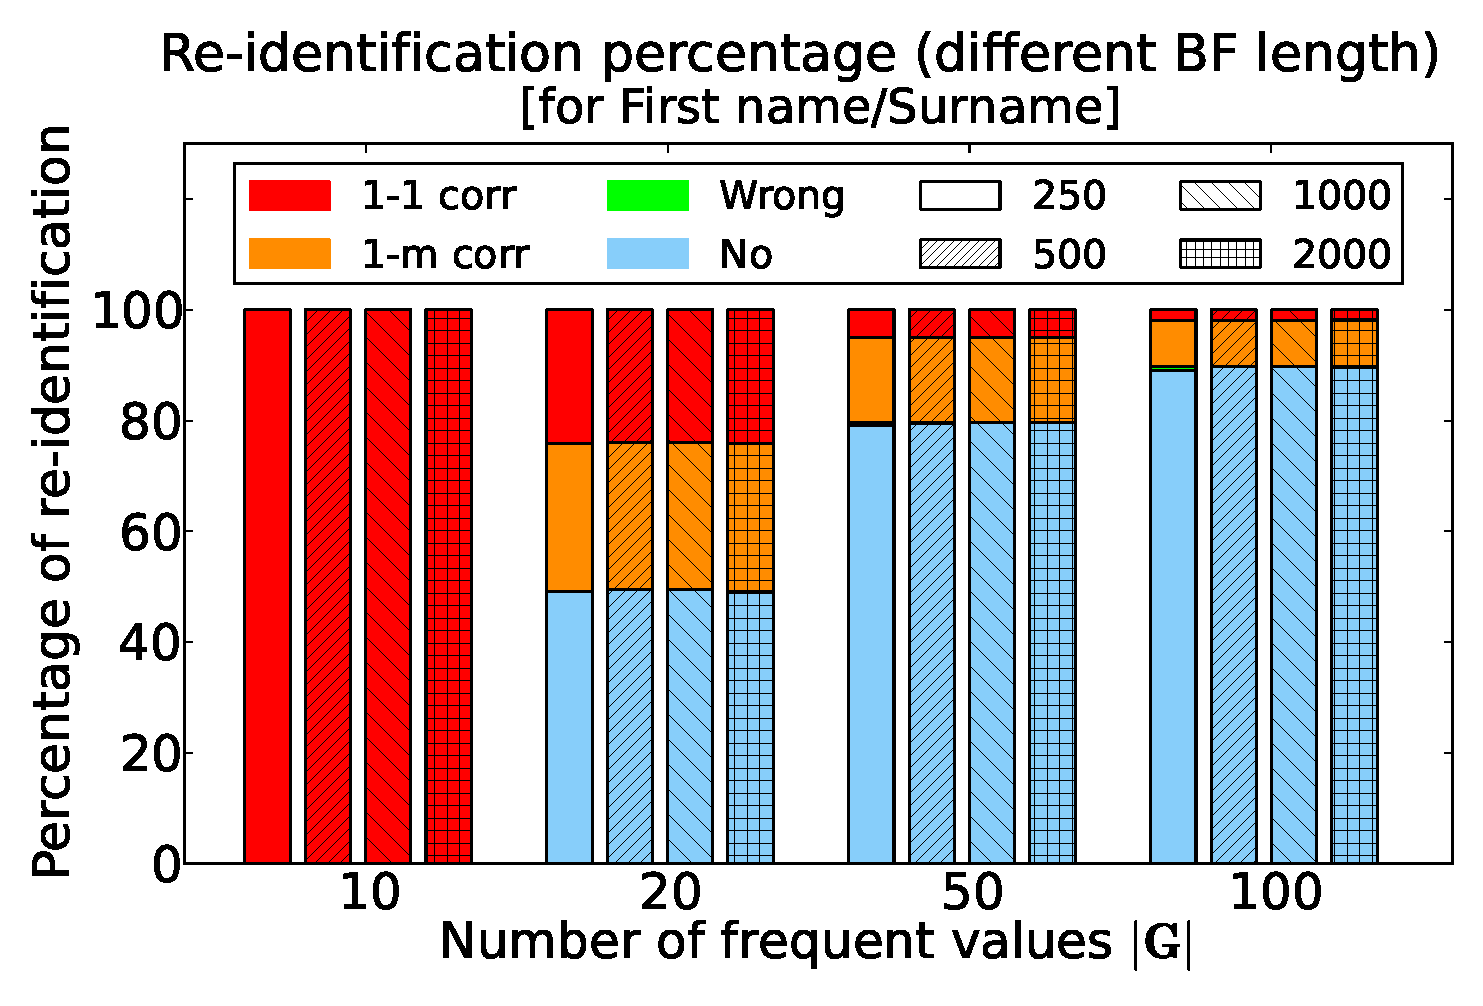
\includegraphics[width=0.31\textwidth]
    {reident-bf_len-1851_allcleaned_1901_allcleaned_5-6}
  ~~
  \includegraphics[width=0.31\textwidth]
    {reident-hash_type-1851_allcleaned_1901_allcleaned_5-6}
  ~~
  \includegraphics[width=0.31\textwidth]
    {reident-bf_harden-1851_allcleaned_1901_allcleaned_5-6}
  \caption{Results for the UKCD data sets with first name (top) and
  combination of first and surname (bottom) for different BF lengths
  (left), different hashing methods (middle), and different BF
  hardening methods (right).
  \label{fig:ukcd}}
\end{figure}

We implemented our attack using Python 2.7 and ran all experiments on
a server with 64-bit Intel Xeon 2.4 GHz CPUs, 128 GBytes of memory
and running Ubuntu 14.04. The programs and data sets are available
from the authors. 

%Toto: generate a similar figure for UKCS? add data set table
%(num rec, attributes use?, num matches? what do we need?
%discuss data sets, table with details - UKC, NCVR balanced,
%NVR 2011 to 2016 (select
%a few, give number of records, number of values in selected attributes)
%show plots with freq distributions of 3 selected attribute values
%(first name, last name, postcode, city?) and their corresponding BF distributions
%If room, show for different data sets.
%experimental setup
%also show if possible for pairs of attributes mapped into 1 BF

\smallskip

\textbf{Discussion:}~
In Fig.~\ref{fig:ncvr} we show the results for the NCVR data sets.
% for one individual attribute (first name) in the top row, and
%three individual attributes (first name, last name, and address in
%the first three rows, respectively), and
%combined attributes of first and surnames in the bottom row.
% BFs are hardened using the balanced method.
%
As can be seen, when the BF length $l$ increases (left column) the
percentage of correct re-identifications mostly increases, as with
larger $l$ the number of q-grams mapped to a certain bit position
decreases. All values can be correctly re-identified for individual
attributes
%nearly $90\%$ of values can be correctly re-identified
%%as 1-to-1 or 1-to-many matches
when the number of frequent values is 10.
%or 20. 
Around half of all
values can still be re-identified even when values from two
attributes are combined.
%
The middle column
%in Fig.~\ref{fig:ncvr}
shows that random hashing
(which supposedly improves privacy on BFs compared to double
hashing~\cite{Kro15,Nie14}) does not provide improved protection
against our attack, as a similar percentage of values can be
correctly re-identified for both hashing approaches. As for using
different values of $q$ (right column)
%in Fig.~\ref{fig:ncvr}),
the accuracy of an attack somewhat improves when $q$ is increased
because larger values of $q$ result in more unique q-grams.

The accuracy results for the UKCD data sets are shown in
Fig.~\ref{fig:ukcd} for the same attributes as for the NCVR data
sets. Similar re-identification patterns as with the NCVR data sets
can be seen for different BF lengths (left) and hashing methods
(middle). We also study how different BF hardening methods affect the
re-identification accuracy, as shown in the right column plots in
Fig.~\ref{fig:ukcd}. For the single attribute case (top right),
neither of the hardening techniques is capable of reducing the
re-identification accuracy, however for the combined attribute
case both hardening techniques improve the privacy of BF encoding.

\begin{table}[!t]
 %\addtolength{\tabcolsep}{-3pt}
  \caption{Comparison of re-identification results with existing BF
     attack methods.}
     \label{table:exist_approaches}
  \centering
  \begin{scriptsize}
    \begin{tabular}{llccc}
    \hline\noalign{\smallskip}
   Publication & Data set & Num BFs~ & ~1-1 corr~ & Run time
     \\ \noalign{\smallskip}\hline\noalign{\smallskip}
  Kuzu et al. (2011)~\cite{Kuz11} & NCVR first names & 3,500 & 400 &
    1,000 sec \\
  Kuzu et al. (2013)~\cite{Kuz13} & Patient names & 20 & 4 & 
    few sec \\
  ~~~~ " & ~~~~ " & 42 & 0 & $>$ week \\
  Niedermeyer et al. (2014)~\cite{Nie14}~ & German surnames & 7,580 &
    934 & $>$ days  \\
  Kroll and Steinmetzer (2015)~\cite{Kro15}~ & German names and
    locations & 100K & 44K & $>$ days \\
  Our approach & NCVR first names & 10--100 & 7--10 & 0.73--0.75 sec
    \\
  ~~~~ " & NCVR first and surnames & 10--100 & 3--6 & 1.5--1.9
  sec  \\
%  ~~~~ " & UKCD surname and address~ & 10 & 10 & 0.05 sec \\
  \noalign{\smallskip} \hline
  \end{tabular}
  \end{scriptsize}
\end{table}

% -------------------
%DV: Peter, for your question on what is the difference between 2 and
%3 in table 1:
%In that paper they first tried to re-identify 40 most frequent
%values ant it took more than a week without any results (0 
%re-identification percentage), and then they used 2 most frequent
%names and it results in 20% (i.e. 4 values are re-identified)
%accuracy in few seconds (they didn't mention the actual number of
%seconds).
%
%That's why I included both entries in the table to show the %scalability of our proposed approach.

% --------------

In Table~\ref{table:exist_approaches} we compare our attack method
with existing approaches in terms of accuracy and efficiency (with
results taken from the corresponding papers). As can be seen, our
method is both more efficient and effective in re-identification,
having both higher accuracy and reduced computational requirements.
% than existing approaches.

These results show the vulnerability of basic BF encoding to our
novel attack. They highlight the need for improved hardening
techniques to overcome such attacks. Our attack provides data
custodians with an efficient method to evaluate the privacy of their
BF encoded databases before using them for PPRL.

\smallskip
\textbf{Recommendations:}~
As a set of guidelines for the practical application of BF based PPRL
systems, to limit the vulnerability of such systems to known attack
methods we recommend to use record-level BF encoding (CLK or RBF),
apply advanced BF hardening methods~\cite{Sch16}, and reduce the
frequency of bit patterns (for example, by salting) to prevent any
frequency analysis.

% --------------------------------------------------------------------

\section{Conclusions and Future Work}
\label{sec-concl}

We have presented a novel efficient frequency-based attack on Bloom
filters (BFs) that contain encoded sensitive attribute values
intended for privacy-preserving record linkage (PPRL). Unlike earlier
attacks on BFs for PPRL, our approach only requires an attacker to
have access to a public database of attribute values, but no
information about the BF encoding used.
%Most importantly, it is independent of the kind of hash function
%used for BF encoding.
Our approach is faster than earlier attacks, making it feasible for
database owners to efficiently validate the security of their
encoded sensitive databases before they are being sent to other
parties for conducting PPRL. We believe our attack is an important 
component to making PPRL more secure for practical applications.

As future work we will study how our approach can be modified for
attacking composite and record-level BFs. We also plan to investigate
the risk of re-identification when advanced hardening techniques, such
as BLIP or BF salting, have been applied. Finally, our attack can be
accelerated by further analyzing the re-identified attribute values,
while correlations between $1$-bits and q-gram sets across BFs could
be identified using association rule mining
techniques~\cite{Ceg06}.

% --------------------------------------------------------------------

%\section*{Acknowledgments}
%
%Peter Christen was supported by a grant from the Simons Foundation.
%The authors would also like to thank the Isaac Newton Institute for
%Mathematical Sciences, Cambridge, for support and hospitality during
%the programme \emph{Data Linkage and Anonymisation} where this work
%was conducted (EPSRC grant EP/K032208/1). This work was partially
%funded by the Australian Research Council under Discovery Project
%DP130101801.

% --------------------------------------------------------------------

%\bibliographystyle{abbrv}
\bibliographystyle{splncs03}
\bibliography{paper} 

\end{document}

% ====================================================================
